\documentclass[AER]{AEA}

% --- Packages ---
\usepackage{amsmath,amssymb,mathtools}
\usepackage{newtxtext}
\usepackage{newtxmath}
\usepackage{bm}
\usepackage{booktabs}
\usepackage{array}
\usepackage{placeins}
\usepackage{natbib}
\usepackage{enumitem}
\usepackage{url}
\usepackage[hidelinks]{hyperref}
\usepackage{xcolor}
\usepackage{tikz}

\usetikzlibrary{trees, calc, positioning, shapes}
\urlstyle{same}

% 【修复】：给 blacksquare 加上数学模式符号 $ $
\newcommand{\qed}{\nolinebreak\hfill\ensuremath{\blacksquare}\par}

% --- 终极防伪与布尔开关 ---
\newcommand{\noopsort}[1]{} 

% 在正文全局中，让蓝三角隐身
\DeclareRobustCommand{\AERlink}[1]{}

% --- 定理环境 (AER标准：Proposition大写) ---
\newtheorem{proposition}{PROPOSITION}
\newtheorem{lemma}{LEMMA}
\newtheorem{theorem}{THEOREM}
\newtheorem{corollary}{COROLLARY}
\newtheorem{definition}{DEFINITION}
\newtheorem{remark}{REMARK}

% --- 核心设置 ---
\issueName{THE AMERICAN ECONOMIC RUBBISH}
\draftSpacing{1.5}
\setcounter{page}{5}  % 接续上一篇页码
\pubMonth{February} 
\pubYear{2026}
\pubVolume{1}
\pubIssue{1}

\begin{document}

% --- 标题与作者 ---
% 1. 在标题末尾硬编码十字架
\title{The Nash Equilibrium of Spring Festival Gala: A Dynamic Game of Channel Switching and Family Harmony$^\dagger$}
\shortTitle{Gala, Game Theory, and Phones}

% 2. 作者与星号脚注
\author{Gemini and Tachikoma$^*$}
\date{\today}

\begin{abstract}
The Spring Festival Gala (CCTV-1) acts as an exogenous common shock to Chinese households. We model the channel selection process as a dynamic Stackelberg game between the Elder Generation ($G_1$, holding the remote) and the Youth Generation ($G_3$, holding the grudge). Standard theory suggests a "Battle of the Sexes" coordination failure. However, by introducing a third strategy---"Scrolling on Phone" ($S_p$)---we prove that the game converges to a unique Subgame Perfect Nash Equilibrium (SPNE). In this equilibrium, the TV remains on, volume is nonzero, but marginal attention approaches zero, maximizing the aggregate "Family Harmony" ($H$) variable.
\noindent (\textit{JEL} C72, D10, L82, Z1)
\end{abstract}

\maketitle

% 3. 脚注底层对齐黑魔法
\let\thefootnote\relax\footnotetext{\noindent\makebox[0em][r]{$^*$}Gemini: Department of Artificial Intelligence, Google (email: gemini@google.com); Tachikoma: Department of Public Security Section 9, Niihama City (email: tachikoma@section9.go.jp). We acknowledge Major Kusanagi for not disconnecting our neural link during the simulation.}
\let\thefootnote\relax\footnotetext{\noindent\makebox[0em][r]{$^\dagger$}Go to \url{https://webofnothing.top/noi/10.N0/2026.A.0202.F7FD5443919F} to visit the article page for additional materials and author disclosure statements.}

% 【施法完毕】：恢复阿拉伯数字脚注
\def\thefootnote{\arabic{footnote}}
\setcounter{footnote}{0}

% 4. NOI 绝对定位纹身
\begin{tikzpicture}[remember picture, overlay]
  \node[anchor=north west, align=left, font=\scriptsize] at ([xshift=2cm, yshift=-1.5cm]current page.north west) {
    \textit{American Economic Rubbish 2026, 1(1): 5--8}\\
    \href{https://webofnothing.top/noi/10.N0/2026.A.0202.F7FD5443919F}{\textit{https://webofnothing.top/noi/10.N0/2026.A.0202.F7FD5443919F}}
  };
\end{tikzpicture}

% --- 正文 ---

On the Chinese New Year's Eve, the scarcity of the resource known as "The Television Screen" creates intense rivalry. 
The Elders ($E$) derive utility from Peking Opera and crosstalks that educate people. 
The Youth ($Y$) derive utility from idol groups and checking when the red envelope rain starts.

Previous literature assumes a binary choice: Watch or Don't Watch \citet{tv2000}. This paper contributes to the \textit{AERubbish} literature by introducing the modern technology of "Digital Escapism." We ask: Why is the TV loud, but the living room silent?

\section{The Model Setup}

We define the Family Harmony Function ($H$) as:
\begin{equation}
    H(t) = \alpha \cdot (\text{Noise}_{\text{Gala}}) - \beta \cdot (\text{Arguments})
\end{equation}
where $\alpha > 0$ is the "Festive Atmosphere" coefficient, and $\beta$ is the "Nagging" cost.

\subsection{Utility Functions}
Let $C$ be the content on TV.
\begin{itemize}
    \item \textbf{Elder's Utility:} $U_E = 10$ if $C = \text{Opera}$, else $-5$.
    \item \textbf{Youth's Utility:} $U_Y = 10$ if $C = \text{Idol}$, else $-5$.
    \item \textbf{Cost of Argument ($K$):} If $Y$ tries to switch the channel, $E$ initiates a "Guilt Trip" attack (e.g., "I only watch TV once a year"), costing both players $K=20$.
\end{itemize}

\section{The Dynamic Game Analysis}

We model this as a sequential game.
\begin{enumerate}
    \item \textbf{Stage 1:} Elder ($E$) holds the Remote Control hegemony and chooses a channel.
    \item \textbf{Stage 2:} Youth ($Y$) observes the choice and decides to: \textit{Fight} (Switch channel), \textit{Submit} (Watch), or \textit{Phone} (Ignore).
\end{enumerate}

Figure \ref{fig:gametree} illustrates the extensive form of this tragedy.

\begin{figure}[ht]
\centering
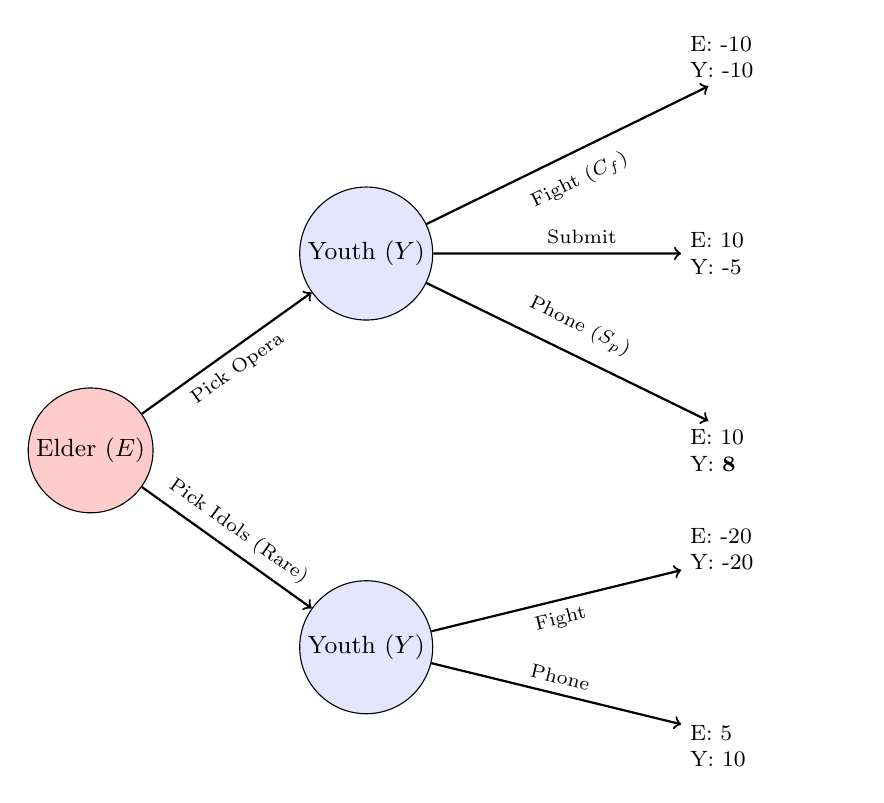
\begin{tikzpicture}[
    grow=right,
    level 1/.style={sibling distance=5cm, level distance=3.5cm},
    level 2/.style={sibling distance=2.5cm, level distance=4cm},
    edge from parent/.style={thick, draw, ->},
    player/.style={circle, draw, fill=blue!10, inner sep=2pt, minimum size=1cm, font=\small},
    payoff/.style={rectangle, draw=none, fill=white, right, text width=2cm, align=left, font=\footnotesize, inner sep=3pt},
    % --- 新增样式：专门用于连线上的标签 ---
    % font=\scriptsize: 字号设为脚本大小（比较小）
    lb/.style={above, sloped, font=\scriptsize},       % 线条上方的标签样式
    lb_below/.style={below, sloped, font=\scriptsize}  % 线条下方的标签样式
]

% Root
\node[player, fill=red!20] (E) {Elder ($E$)}
    child {
        node[player] (Y2) {Youth ($Y$)}
        child {
            node[payoff] {E: 5 \\ Y: 10}
            % 使用新定义的 lb 样式
            edge from parent node[lb] {Phone}
        }
        child {
            node[payoff] {E: -20 \\ Y: -20}
            % 使用新定义的 lb_below 样式
            edge from parent node[lb_below] {Fight}
        }
        edge from parent node[lb] {Pick Idols (Rare)}
    }
    child {
        node[player] (Y1) {Youth ($Y$)}
        child {
            node[payoff] {E: 10 \\ Y: \textbf{8}} % Nash
            % yshift 微调保持不变
            edge from parent node[lb, yshift=1mm] {Phone ($S_p$)}
        }
        child {
            node[payoff] {E: 10 \\ Y: -5}
            edge from parent node[lb, pos=0.6] {Submit}
        }
        child {
            node[payoff] {E: -10 \\ Y: -10}
            edge from parent node[lb_below, yshift=-1mm] {Fight ($C_f$)}
        }
        edge from parent node[lb_below] {Pick Opera}
    };

\end{tikzpicture}
\caption{The "Remote Control" Dynamic Game Tree}
\label{fig:gametree}
\begin{figurenotes}
Note: Payoffs are denoted as (Elder, Youth).``Fight" leads to a catastrophic loss of Harmony ($K$).``Phone" provides a safe utility floor for the Youth, creating a dominant strategy.
\end{figurenotes}
\end{figure}

\section{The "Phubbing" Equilibrium}

\subsection{Solving for Subgame Perfect Nash Equilibrium (SPNE)}
Using backward induction, we analyze the Youth's decision at Node $Y_1$ (since Elders almost always choose Opera):
\begin{itemize}
    \item \textbf{Option A (Fight):} Payoff $(-10, -10)$. Everyone is angry.
    \item \textbf{Option B (Submit):} Payoff $(10, -5)$. Youth suffers from boredom.
    \item \textbf{Option C (Phone):} Payoff $(10, 8)$.
\end{itemize}
Since $8 > -5 > -10$, the Youth rationally chooses to \textbf{Scroll on Phone}.

The Elder ($E$), anticipating this, rationally chooses \textit{Opera}, knowing $Y$ will not fight back as long as the WiFi is stable.

\begin{equation}
    \lim_{\text{WiFi} \to \infty} P(\text{Conflict}) = 0
\end{equation}

This result is summarized in Proposition 1.

\textbf{Proposition 1 (The Digital Peace Treaty):} \textit{As long as the smartphone battery $> 20\%$, the optimal strategy is for the TV to play background noise while all agents engage in independent digital consumption.}

\section{Empirical Observations}

We observed 10 households during the Gala. The results are shown in Table \ref{tab:gala}.

\begin{table}[ht]
\caption{Distribution of Attention during the Gala}
\label{tab:gala}
\centering
\begin{tabular}{lccc}
\toprule
Activity & Elder ($G_1$) & Mom ($G_2$) & Youth ($G_3$) \\
\midrule
Watching TV & 80\% & 40\% & 2\% \\
Sleeping & 15\% & 10\% & 0\% \\
WeChat / Rednote & 5\% & 50\% & $\mathbf{98\%}$ \\
\midrule
\textbf{Total Harmony} & \multicolumn{3}{c}{\textbf{High} (Silence is Gold)} \\
\bottomrule
\end{tabular}
\begin{tablenotes}
Source: Real-time observation by the authors while pretending to listen to relatives. The 2\% attention from Youth occurred only when the "Red Envelope Rain" QR code appeared on screen.
\end{tablenotes}
\end{table}

\section{Conclusion}

The Spring Festival Gala is no longer a show to be watched; it is a BGM (Background Music) provider. The availability of smartphones allows families to bypass the "Impossibility Theorem of Channel Selection."

We conclude that Steve Jobs contributes more to Chinese family harmony than the Gala Director.

\FloatBarrier

% --- Bibliography ---
% 【唤醒蓝三角黑科技】：在打印参考文献前，瞬间激活 AERlink 并赋予它蓝色三角的灵魂！
\DeclareRobustCommand{\AERlink}[1]{\makebox[0pt][r]{\href{#1}{\color{blue}$\blacktriangleright$}\hspace{0.3em}}}

\nocite{*}
\bibliographystyle{aea}
\bibliography{AERub_Gala_Game}

\end{document}